\documentclass[12pt, twoside, a4paper]{article}

\usepackage[margin=1truein]{geometry}
\usepackage{amsmath}
\usepackage{amssymb}
\usepackage{graphicx}
\usepackage[figurename=Slika,labelfont=bf]{caption}
\usepackage{tabularx}
\usepackage{mathtools}
\usepackage{pdflscape}
\usepackage{rotating}

\usepackage[dvipsnames]{xcolor}

\definecolor{darkblue}{rgb}{0, 0, 0.4}
\usepackage[
  colorlinks = true,
  urlcolor = darkblue,
  linkcolor = black
]{hyperref}

\usepackage{qrcode}

%\usepackage[answerdelayed,lastexercise]{exercise}

\DeclareGraphicsRule{*}{mps}{*}{}

\input serbian

\renewcommand*\contentsname{Sadr{\zv}aj}

\usepackage{titlesec}
\newcommand{\sectionbreak}{\clearpage
  \vskip 0.75in plus 0.25in minus 0.25in\relax}
%\newcommand{\subsectionbreak}{\clearpage}

\def\K{\mathop{\vcenter{\hbox{\rm\huge K}}}\limits}
\def\n{n}
\def\Ki{\K_{\n=1}}
\def\Kinf#1#2{\Ki^\infty\displaystyle{\frac{#1}{#2}}}

\def\mul{{\cdot}}
\def\navod#1{\relax,\kern-0.06667em,\relax#1\relax``\relax}

\def\logten{\log_{10}}
\def\logtwo{\log_2}
\def\loga{\log_a}
\def\logb{\log_b}
\def\puta{\times}
\def\comma{{,}}
\let\dotacc=\.
\def\.{{,}}
%\def\e{{\boldsymbol{e}}}
\def\e{{\bf e}}
%\def\naplog{\mathop{\mathop{\rm Log}\limits^{\rm Nap}}\nolimits}
\def\naplog{\mathop{\rm NapLog}\nolimits}
\def\QED{\ensuremath{\qquad\square}}
\def\th{t_{1/2}}
\def\um#1{\,{\rm#1}}
\newdimen\mm \mm=1truemm

\def\ram#1{\,\fcolorbox{black}{white}{$\displaystyle{\mathstrut #1}$}\,}
\def\okvir#1{\,\fcolorbox{black}{Goldenrod}{$\displaystyle{\mathstrut #1}$}\,}
\def\sledi{{\quad\Rightarrow\quad}}

\newcount\exno \exno=0
\def\zabox#1{\leavevmode\hbox to 5em{{\bf #1}\hfill}}
\def\ans{\par\medskip\noindent\zabox{Re{\sv}e{\nj}e:}}
\def\zad{\global\advance\exno by 1\relax
  \par\noindent\leavevmode
  \llap{$\vartriangleright\>$}\zabox{Zadatak:}}
\newcommand{\rsinfty}{{\,\widetilde{\!\infty\!}\,}}

\def\footnote#1{\relax}


\begin{document}

\begin{titlepage}
\setcounter{page}{0}
\thispagestyle{empty}
\begin{center}
\large
Gimnazija \navod{Bora Stankovi{\cc}}\\
Ni{\sv}, Srbija\\
\vfill
\LARGE
\textbf{MATURSKI RAD}\\
\Large
\bigskip
Predmet: Matematika\\
\smallskip
Tema: Logaritam\\
\large
{\it jedna{\cv}ine i nejedna{\cv}ine}\\
%(jedna{\cv}ine i nejedna{\cv}ine)\\
\vfill\vfill
\begingroup
\large
\setbox0=\hbox{Luka Ne{\sv}i{\cc}, IV/\,6}%
\begin{tabularx}{\textwidth}{lXl}
\rule{\wd0}{0pt}&&\rule{\wd0}{0pt}\\
U{\cv}enik:&&Profesor:\\
\copy0&&Nenad Toti{\cc}\\
%\noalign{\bigskip}
%\rule{\wd0}{0.2pt}&&\rule{\wd0}{0.2pt}\\
\end{tabularx}
\endgroup
\vskip 2truecm
\normalsize
\the\year.
\end{center}
\end{titlepage}


\tableofcontents


\section{Uvod}


\subsection{Definicija logaritma}

Ako je
$$
x=b^y
$$
onda se mo{\zv}e pisati
\begin{equation}
\okvir{y=\log_b x},
\end{equation}
gde je $b$ {\sl osnova\/} ({\sl baza\/}) logaritma, a $x$ {\sl argument}.
(Izgovara se \navod{$y$ je jednako logaritam od $x$ za osnovu $b$}
ili kra{\cc}e \navod{$y$ je logaritam $b$ od $x$}.)
Tako{\dj}e va{\zv}i
$$
b=x^{1/y}=\sqrt[y]x.
$$
Sama re{\cv} {\sl logaritam\/} poti{\cv}e od gr{\cv}kih re{\cv}i 
$\lambda\acute o\gamma o\varsigma$~({\sl logos\/}) i 
$\acute\alpha\rho\iota\theta\mu\acute o\varsigma$~({\sl aritmos\/}), 
sa zna{\cv}e{\nj}em \navod{broj kojim se ra{\cv}una}.

\subsection{Grafik funkcije}

\newcounter{figno}
\def\slika#1#2{\stepcounter{figno}%
\displaylines{
\hbox{#1}\cr
\hbox{{\bf Slika \thefigno:\/~}#2}}}


Funkcija je u skupu realnih brojeva ${\mathbb R}$ definisana za $x>0$ i $b>0\land b\ne1$.
Za $b>1$ funkcija je rastu{\cc}a, dok je za $b<1$ funkcija opadaju{\cc}a.
Funkcija ima samo jednu {\sl nulu}, uvek za $x=1$.
Va{\zv}i {\sl bijekcija\/}: 
$\logb x=\logb y \Leftrightarrow x=y$.
$$
\slika{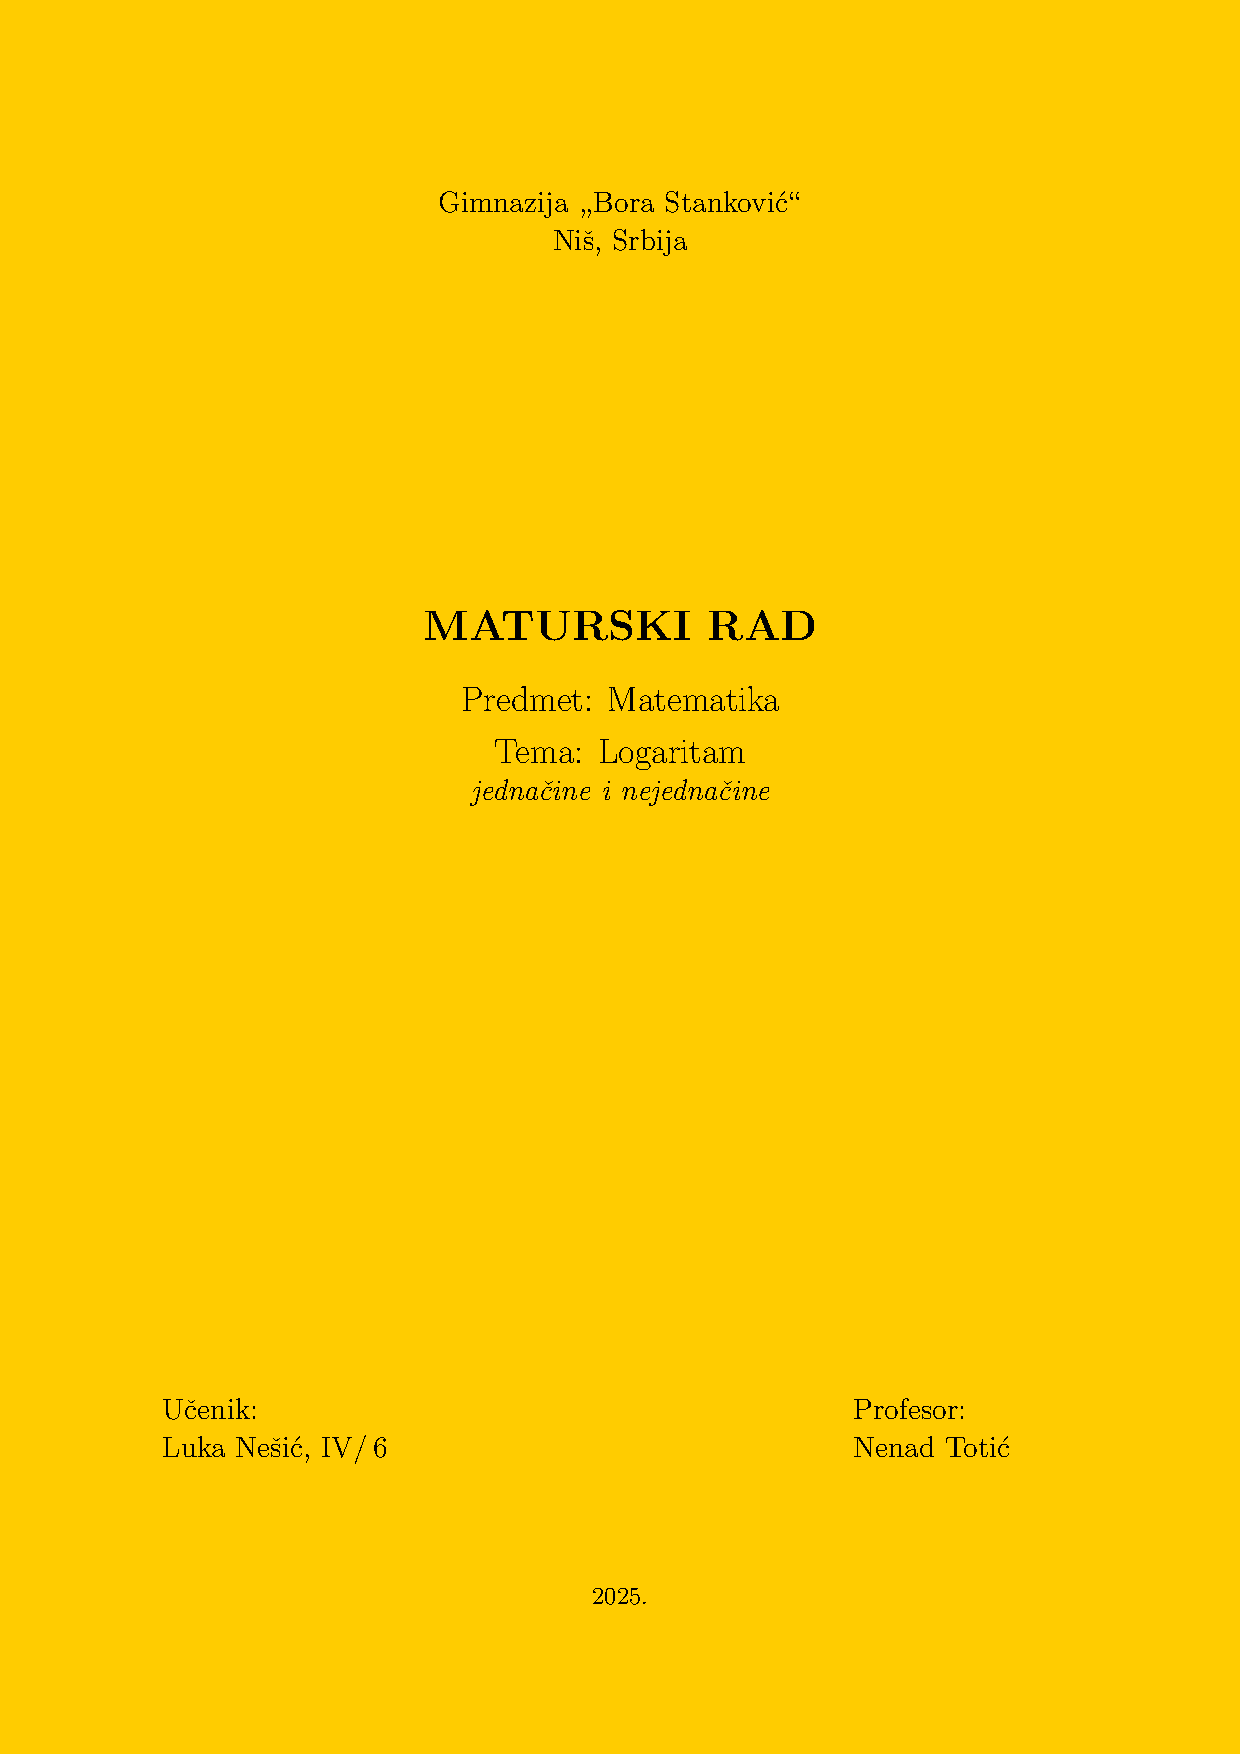
\includegraphics[]{log.1}}{Grafik logaritamske funkcije $y=\logb x$.}
$$

\subsection{Antilogaritam}

\def\antilog{\mathop{\rm antilog}\nolimits}
Inverzna funkcija logaritmu
je obi{\cv}no stepenova{\nj}e osnove logaritma argumentom i zove se {\sl antilogaritam}
\begin{equation}
\okvir{\antilog_bx = \logb^{-1}x =  b^x}.
\end{equation}
Iz same definicije va{\zv}i
\begin{equation}
\okvir{\log_b(\antilog_b x)=\antilog_b(\log_b x)=x}.
\end{equation}



\section{Jednakosti}

\subsection{Logaritam stepena osnove}

Po samoj definiciji logaritma, ako je $x=b^a$, onda je
\begin{equation}
\okvir{\logb b^a=a}.
\label{eq:powb}
\end{equation}
Ako stavimo da je $1=b^0$, odnosno, $b=b^1$, dobijamo da je
\begin{equation}
\okvir{\logb 1=0}\qquad\text{i}\qquad\okvir{\logb b=1}.
\end{equation}
Tako{\dj}e je bitna jednakost
\begin{equation}
\okvir{b^{\logb x}=x}
\end{equation}
koja proizilazi iz same definicije logaritma i antilogaritma.

\subsection{Logaritam proizvoda}

Ako je
$$
u=\logb x\land v=\log_b y \sledi x=b^u\land y=b^v,
$$
onda je
$$
x\cdot y=b^ub^v=b^{u+v}\sledi \logb(x\cdot y)=\logb b^{u+v}=u+v.
$$
Odavde je
\begin{equation}
\okvir{\logb(x\cdot y)=\logb x+\logb y}.
\label{eq:lnmul}
\end{equation}

Iz ove jednakosti se mo{\zv}e izvesti formula za logaritam faktorujela broja. Ako je
$$
n!=\prod_{k=1}^n k\sledi \log(n!)=\sum_{k=1}^n\log k.
$$
(Zanim{\lj}ivo je da je $\log(1\cdot2\cdot3)=\log(1+2+3)=\log1+\log2+\log3$.)


\subsection{Logaritam koli{\cv}nika}

Sli{\cv}no logaritmu proizvoda, 
ako je
$$
u=\logb x\land v=\log_b y \sledi x=b^u\land y=b^v,
$$
onda je
$$
x/ y=b^ub^{-v}=b^{u-v}\sledi \logb(x/y)=\logb b^{u-v}=u-v.
$$
Odavde je
\begin{equation}
\okvir{\logb(x/ y)=\logb x-\logb y}.
\label{eq:lndiv}
\end{equation}
Iz ove jednakosti sledi
\begin{equation}
\okvir{\logb(1/x)=-\logb x}.
\label{eq:recip}
\end{equation}

\subsection{Logaritam stepena broja}

Ako je
$$
y=x^n=\underbrace{x\cdot x\cdots x}_{\text{$\mathstrut n$ puta}},
$$
onda, iz jednakosti za logaritam proizvoda \eqref{eq:lnmul}, sledi da je
$$
\logb y=\logb (\underbrace{\mathstrut x\cdot x\cdots x}_{\text{$n$ puta}})
=\underbrace{\mathstrut \logb x+\logb x+\cdots+\logb x}_{\text{$n$ puta}}
=n\logb x,
$$
odakle je
\begin{equation}
\okvir{\logb x^n=n\logb x}.
\label{eq:bpow}
\end{equation}
Iz ove jednakosti mo{\zv}e se izvesti i jednakost
\begin{equation}
\okvir{\logb\sqrt[n] x={1\over n}\logb x}.
\label{eq:lnroot}
\end{equation}
Odavde se mo{\zv}e izvesti jednakost
\begin{equation}
\okvir{x^y=b^{y\logb x}}.
\label{eq:power}
\end{equation}


\subsection{Promena osnove logaritma}

Ako je
$$
y = \loga x\sledi x = a^y,
$$
onda je 
$$
\logb x=\logb a^y=y\logb a=\loga x\cdot\logb a.
$$
Odavde je
\begin{equation}
\okvir{\loga x={\logb x\over\logb a}}.
\label{eq:chgbase}
\end{equation}
Iz ove jednakosti, ako stavimo da je $x=b$, se dobija i jednakost
\begin{equation}
\okvir{\loga b\cdot\logb a = 1}.
\end{equation}
Iz jednakosti \eqref{eq:powb} i \eqref{eq:chgbase}, ako stavimo da je $a=b^n$, sledi jednakost
\begin{equation}
\okvir{\log_{b^n}x = {1\over n}\logb x}.
\label{eq:powbase}
\end{equation}
Odavde, ako stavimo da je $n=-1$, sledi
\begin{equation}
\okvir{\log_{1/b}x = -\logb x},
\end{equation}
a uzev{\sv}i u obzir i jednakost \eqref{eq:recip} dobija se
\begin{equation}
\okvir{\log_{1/b}x = \logb(1/x)}.
\end{equation}



\section{Naj{\cv}e{\sv}{\cc}e logaritamske osnove}

\subsection{Osnova 10}

U ini{\zv}e{\nj}erstvu se naj{\cv}e{\sv}{\cc}e koristi osnova logaritma 10,
zove se {\sl dekadni\/} ili {\sl zajedni{\cv}ki\/} logaritam, i pi{\sv}e se
$$
y=\logten x
$$
ili, skra{\cc}eno,
$$
y=\lg x.
$$
Ponekad se mo{\zv}e videti i samo
$$
y=\log x,
$$
bez navo{\dj}e{\nj}a osnove, ali treba obratiti pa{\zv}{\nj}u na kontekst.
Ako je neki in{\zv}e{\nj}erski tekst u pita{\nj}u, najverovatnije se misli na osnovu 10.

Dekadni logaritam je pogodan i kada se koristi, takozvani {\sl nau{\cv}ni\/} ili {\sl in{\zv}e{\nj}erski\/}
zapis broja.
Na primer, {\sl Plankova konstanta\/} (Max Planck) iznosi
$$
h=6\.62607015\puta 10^{-34}
$$
koja ima dekadni logatiram
$$
\logten h=\logten(6\.62607015) - 34.
$$

U fizici se za mere{\nj}e nivoa signala ili zvuka koristi jedinica {\sl be\/l}~(B), ali je {\cv}e{\sv}{\cc}e
u prakti{\cv}noj upotrebi 10 puta ma{\nj}a jedinica {\sl decibel\/}~(dB), odnosno, $1\um{B}=10\um{dB}$. \
Nivo \hbox{sig\-na\-la} $L$, koji zavisi
od odnosa izmerene snage $P$ i refrentne snage $P_0$, izra{\zv}en u deci\-belima iznosi
$$
L=10\logten\left({P\over P_0}\right)\um{dB}.
$$
Kako se u akustici uzima da je referentna snaga $P_0=10^{-12}\um W$, moglo bi se pisati
da je nivo zvuka u decibelima
$$
L=10\logten(P)-120.
$$

Normalan govor je oko $50\um{dB}$, 
zvuk motora mlaznog aviona pri poleta{\nj}u je $150\um{dB}$, 
%raketa Saturn~V oko $220\um{dB}$,
a smrtonosan je zvuk od $240\um{dB}$ i vi{\sv}e.
Zvu{\cv}ni top {\sf Genasys LRAD} ima nivo zvuka od oko $160\um{dB}$,
{\sv}to zna{\cv}i da je $10^{11}$ puta mo{\cc}niji od govora.

Sli{\cv}na formula se koristi i za odre{\dj}iva{\nj}e ja{\cv}ine zem{\lj}otresa.

\subsection{Osnova 2}

\def\lb{\mathop{\rm lb}}
\def\bits{{\it bits}}
\def\mant{{\it mantisa}}%
\def\expo{{\it eksponent}}%
\def\znak{{\it znak}}%

U informatici se {\cv}esto koristi logaritam sa osnovom 2, koji se zove {\sl binarni\/} logaritam,
i pi{\sv}e se
$$
y=\logtwo x
$$
ili, skra{\cc}eno,
$$
y=\lb x.
$$
Koristi se u kombinatorici, kao i u odre{\dj}iva{\nj}u {\sl koli{\cv}ine informacija},
odnosno, potrebnog broja bitova me\-mo\-ri\-je za sme{\sv}ta{\nj}e nekog podatka.
Ako se zna da {\cc}e u me\-mo\-ri\-ju biti upisivani celi brojevi od 0 do $n$, onda je potrebno rezevisati
$$
\bits = \lfloor\logtwo(n)\rfloor+1
$$
bitova memorije, gde $\lfloor x\rfloor$ predstav{\lj}a {\sl najve{\cc}i ceo broj koji je ma{\nj}i ili jednak} $x$
(izgovara se \navod{najve{\cc}e celo od $x$}). 
Na primer, ako {\cc}e u odre{\dj}enoj memoriji najve{\cc}i 
broj biti milion, onda je za to potrebno rezevisati
$$
\bits=\lfloor\logtwo(1\,000\,000)\rfloor+1=\lfloor 19\.9315685693\rfloor+1 = 19+1=20
$$
bitova memorije. Najve{\cc}i broj koji mo{\zv}e stati u ovih rezervisanih 20 bitova memorije je binarni broj koji ima 20 jedinica
i iznosi 
$$
(1111\,1111\,1111\,1111\,1111)_2=
2^{20}-1=1\,048\,575.
$$

Kako su i realni brojevi u memoriji predstav{\lj}eni kao ure{\dj}eni parovi binarnih brojeva u obliku
$(\mant,\expo)$, sa zna{\cv}e{\nj}em
$$
x=\mant\puta2^\expo,
$$
binarni logaritam bi bio izra{\cv}unat kao
$$
\logtwo(x)=\logtwo(\mant)+\expo,
$$
ako je $\mant>0$, ina{\cv}e je nedefinisan.

\smallskip

Binarni logaritam se koristi i u atomskoj fizici.
Vreme {\sl poluraspada\/} $\th$ je vreme potrebno da se raspadne polovina jezgara atoma neke materije. 
Ako imamo po{\cv}etan broj jezgara $N_0$ i broj jezgara $N_t$ nakon vremena $t$, njihov odnsos
se mo{\zv}e pred\-sta\-vi\-ti formulom
\begin{equation}
\label{eq:halftime}
{N_0\over N_t}=2^{t/\th}\sledi {t\over\th}=\logtwo\left( {N_0\over N_t} \right).
\end{equation}
Ova formula se koristi i za odre{\dj}iva{\nj}e starosti stena ili fosila.


%\clearpage

\subsection{Osnova $\e$}

Ovu logaritamsku osnovu je otkrio Jakob Bernuli (Jacob Bernoulli) kada je
prou{\cv}avao {\sl slo{\zv}enu kamatu}, ali je Ojler (Leonhard Euler) dokazao da je
$$
\e=\lim_{n\to\infty}\left(1+{1\over n}\right)^{\!n}\!,
$$
odredio {\nj}enu vrednosti i dao joj ime.
Logaritam za ovu osnovu se zove {\sl prirodni\/} logaritam ({\sl logarithmus naturalis\/})
i pi{\sv}e se
$$
\ln x=\log_\e x.
$$

\def\ep{\hphantom{!}}
Antilogaritam je $\e^x$, koji se kao funkicja pi{\sv}e $\exp(x)$, i zove se
{\sl eksponencijalna funkcija}. Ova funkcija je poznata po tome {\sv}to je to 
jedina funkcija {\cv}iji je izvod jednak samoj funkciji. Brojna vrednost se mo{\zv}e
izra{\cv}unati formulom
\begin{equation}
\label{eq:exp}
\okvir{\e^x=\exp(x)=\sum_{n=0}^\infty{x^n\over n!}},
\end{equation}
Ako stavimo da je $x=1$,
brojna vrednost osnove prirodnog logaritma $\e$ se mo{\zv}e odrediti
\begin{equation}
\label{eq:e}
\begin{aligned}
\e
&={1\over\ep0!}+{1\over\ep1!}+{1\over\ep2!}+{1\over\ep3!}+{1\over\ep4!}+{1\over\ep5!}+\cdots\\
&=2\.
7182818284\,
5904523536\,
0287471352\,
6624977572\,\ldots
\end{aligned}
\end{equation}
sa {\zv}e{\lj}enom ta{\cv}no{\sv}{\cc}u.


\section{Brojna vrednost}

\subsection{Formula}

Brojna vrednost prirodnog logaritma mo{\zv}e biti izra{\cv}unata pomo{\cc}u formule
\begin{equation}
\okvir{
\ln x
%&=2\mathop{\rm arctanh}\frac{x-1}{x+1}\\
=\sum_{n=0}^\infty\frac{2}{2n+1}\left(\frac{x-1}{x+1}\right)^{\!2n+1}
}.
\label{eq:lnred}
\end{equation}
do {\zv}e{\lj}ene ta{\cv}nosti.
Postupak, kojim se ra{\cv}una $y=\ln x$ sa ta{\cv}no{\sv}{\cc}u $\varepsilon$,
izgleda ovako:
\def\asg{\leftarrow}%
\begin{equation}
\label{eq:alg}
\begingroup\color{Blue}
\begin{aligned}
&r\asg(x-1)/(x+1);\quad k\asg 1;\quad p\asg 2r;\quad q\asg r^2;\quad a\asg p;\quad y\asg a;\\
&\text{ponav{\lj}ati dok je $|a|>\varepsilon$:}\\
&\qquad k\asg k+2;\quad p\asg p\cdot q;\quad a\asg p/k;\quad y\asg y+a;
\end{aligned}
\endgroup
\end{equation}
(Videti zadatak \ref{sssec:ln3} na strani \pageref{sssec:ln3}.)
Ovim na{\cv}inom se mo{\zv}e izra{\cv}unati konstanta
\begin{align*}
\ln2
&=\frac{2}{1\cdot3^1}+\frac{2}{3\cdot3^3}+\frac{2}{5\cdot3^5}+\frac{2}{7\cdot3^7}+\frac{2}{9\cdot3^9}+\cdots\\
\noalign{\smallskip}
&= 0\.
6931471805\,
5994530941\,
7232121458\,
1765680755\,
\ldots\\
\intertext{kao i konstanta}
\ln 10&=2\.
3025850929\,
9404568401\,
7991454684\,
3642076011\,
\ldots
\end{align*}
Ove konstante se koriste prilikom izra{\cv}unava{\nj}a vrednosti binarnog, odnosno, dekadnog logaritma
$$
\lb x=\logtwo x={\ln x\over \ln2},\qquad \lg x=\logten x={\ln x\over \ln 10}.
$$

\subsection{Veri{\zv}ni razlomak}

Brojna vrednost prirodnog logaritma mo{\zv}e se izra{\cv}unati i pomo{\cc}u {\sl veri{\zv}nog razlomka}
\begin{align*}
\ln(1+x)
&=\cfrac{x}{1+\cfrac{1^2x}{2-1x+\cfrac{2^2x}{3-2x+\cfrac{3^2x}{4-3x+\ddots}}}}\\
\noalign{\vskip-3pt}
&=\cfrac{x}{1+ \Kinf{\n^2x}{\n+1-\n x}}.
\end{align*}
Poput simbola koji se koriste za sumu `$\rm\Sigma$' ili proizvod `$\rm\Pi$', 
Gaus (Carl Friedrich Gauss) je smislio, verovatno, najpogodniji na{\cv}in za predstav{\lj}a{\nj}e
veri{\zv}nih (lan{\cv}anih) razlomaka,
gde simbol `K' poti{\cv}e od nema{\cv}ke re{\cv}i za {\sl prekinuti lanac\/} ({\sl Kettenbruch\/}). 
Izraz iza ovog simbola pokazuje kako izgleda {\sl op{\sv}ti {\cv}lan\/} veri{\zv}nog razlomka.

\def\ff#1/#2/{\frac{#1}{#2}}
Ako pomo{\cc}u ove formule izra{\cv}unamo prvih 11 konvergenata $\ln2$ kao $-\ln(1-1/2)$, dobi{\cc}emo
$$
\ln2\approx\ff1/2/, \ff5/8/, \ff2/3/, \ff131/192/, \ff661/960/, \ff1327/1920/, \ff1163/1680/, \ff148969/215040/, 
\ff447047/645120/, \ff44711/64512/, \ff983705/1419264/, \dots
$$
gde je posled{\nj}i razlomak ta{\cv}an na 5 decimala.


\subsection{Logaritamske tablice}

Prve tablice logaritama je izra{\cv}unao Neper (John Napier of Merchiston)
1614.\ godine,
koje su prakti{\cv}no sadr{\zv}ale logaritam za osnaovu $1/\e$, sa skaliranim argumentom i rezultatom,
iako sam Neper nije znao za konstantu $\e$.
Savremenim zapisom bi ovaj logaritam bio definisan kao
$$
\naplog (x) = 10^7\log_{1/\e}(x/10^7) = -10^7\ln(x/10^7).
$$

Nekoliko godina kasnije, 1617.\ i 1624, Brigs (Henry Briggs) je izra{\cv}unao
tablice de\-kad\-nih logaritama sa 14 cifara ta{\cv}nosti, koje se uz dopune i ispravke
koriste i danas pod imenom {\sl Brigsove tablice}.


\subsection{Logaritmar}

\def\hair{}%
\def\extra{}%

\newdimen\px \px=1truein \divide\px by 200
\def\rstrut{\vrule width 0pt height 0.8truemm depth 0pt\relax}
\def\zbox{\hbox to 0pt\relax}
\def\cbox#1{\zbox{\hss#1\hss}}
\def\mark{\cbox{\rstrut\vrule width 1\px}}
\def\ruler#1#2{\zbox{\kern#1\u\cbox{\sf#2}\hss}}
\def\marker#1{\zbox{\kern#1\u\mark\hss}}
\def\nit#1{\zbox{\kern#1\u\cbox{\color{red}\rstrut\vrule width 1\px}\hss}}


\def\std{%
\marker{0}%
\marker{0.30102999566398119521373889472449}%
\marker{0.47712125471966243729502790325512}%
\marker{0.60205999132796239042747778944899}%
\marker{0.69897000433601880478626110527551}%
\marker{0.77815125038364363250876679797961}%
\marker{0.84509804001425683071221625859264}%
\marker{0.90308998699194358564121668417348}%
\marker{0.95424250943932487459005580651023}%
\marker{1}%
\marker{0.4971498726941338543512682882909}% pi
\marker{0.43429448190325182765112891891661}% e
%\marker{0.20898764024997873376927208923756}% phi
%\marker{0.15051499783199059760686944736225}% sqrt 2
%\marker{0.23856062735983121864751395162756}% sqrt 3
%\marker{1.041392685}% 11.00
%\marker{1.079181246}% 12.00
%\marker{0.522878745}% 3.33
\marker{0.63778431130053678912296749864511}% log e
}
\def\half{%
%\marker{1.021189299}% 10.50
%\marker{1.060697840}% 11.50
%\marker{1.096910013}% 12.50
%\marker{1.113943352}% 13.00
\marker{0.17609125905568124208128900853062}% 1.5
\marker{0.39794000867203760957252221055101}% 2.5
\marker{0.54406804435027563549847736386814}% 3.5
\marker{0.65321251377534367937631691178574}% 4.5
\marker{0.74036268949424384553646107651853}% 5.5
\marker{0.81291335664285557399276626321784}% 6.5
\marker{0.87506126339170004686755011380613}% 7.5
\marker{0.92941892571429273332643099960384}% 8.5
\marker{0.97772360528884776632259458103244}% 9.5
}


\def\tenth{%
\marker{-0.045757491}% 0.90
\marker{-0.096910013}% 0.80
\marker{0.041392685}% 1.1
\marker{0.079181246}% 1.2
\marker{0.113943352}% 1.3
\marker{0.146128036}% 1.4
\marker{0.204119983}% 1.6
\marker{0.230448921}% 1.7
\marker{0.255272505}% 1.8
\marker{0.278753601}% 1.9
\marker{0.322219295}% 2.1
\marker{0.342422681}% 2.2
\marker{0.361727836}% 2.3
\marker{0.380211242}% 2.4
\marker{0.414973348}% 2.6
\marker{0.431363764}% 2.7
\marker{0.447158031}% 2.8
\marker{0.462397998}% 2.9
\marker{0.491361694}% 3.1
\marker{0.505149978}% 3.2
\marker{0.518513940}% 3.3
\marker{0.531478917}% 3.4
\marker{0.556302501}% 3.6
\marker{0.568201724}% 3.7
\marker{0.579783597}% 3.8
\marker{0.591064607}% 3.9
\marker{0.612783857}% 4.1
\marker{0.623249290}% 4.2
\marker{0.633468456}% 4.3
\marker{0.643452676}% 4.4
\marker{0.662757832}% 4.6
\marker{0.672097858}% 4.7
\marker{0.681241237}% 4.8
\marker{0.690196080}% 4.9
\marker{0.707570176}% 5.1
\marker{0.716003344}% 5.2
\marker{0.724275870}% 5.3
\marker{0.732393760}% 5.4
\marker{0.748188027}% 5.6
\marker{0.755874856}% 5.7
\marker{0.763427994}% 5.8
\marker{0.770852012}% 5.9
\marker{0.785329835}% 6.1
\marker{0.792391689}% 6.2
\marker{0.799340549}% 6.3
\marker{0.806179974}% 6.4
\marker{0.819543936}% 6.6
\marker{0.826074803}% 6.7
\marker{0.832508913}% 6.8
\marker{0.838849091}% 6.9
\marker{0.851258349}% 7.1
\marker{0.857332496}% 7.2
\marker{0.863322860}% 7.3
\marker{0.869231720}% 7.4
\marker{0.880813592}% 7.6
\marker{0.886490725}% 7.7
\marker{0.892094603}% 7.8
\marker{0.897627091}% 7.9
\marker{0.908485019}% 8.1
\marker{0.913813852}% 8.2
\marker{0.919078092}% 8.3
\marker{0.924279286}% 8.4
\marker{0.934498451}% 8.6
\marker{0.939519253}% 8.7
\marker{0.944482672}% 8.8
\marker{0.949390007}% 8.9
\marker{0.959041392}% 9.1
\marker{0.963787827}% 9.2
\marker{0.968482949}% 9.3
\marker{0.973127854}% 9.4
\marker{0.982271233}% 9.6
\marker{0.986771734}% 9.7
\marker{0.991226076}% 9.8
\marker{0.995635195}% 9.9
}


\def\prec{%
\marker{-0.022276395}% 0.95
\marker{-0.070581074}% 0.85
\marker{-0.004364805}% 0.99
\marker{-0.008773924}% 0.98
\marker{-0.013228266}% 0.97
\marker{-0.017728767}% 0.96
\marker{-0.026872146}% 0.94
\marker{-0.031517051}% 0.93
\marker{-0.036212173}% 0.92
\marker{-0.040958608}% 0.91
\marker{-0.050609993}% 0.89
\marker{-0.055517328}% 0.88
\marker{-0.060480747}% 0.87
\marker{-0.065501549}% 0.86
\marker{-0.075720714}% 0.84
\marker{-0.080921908}% 0.83
\marker{-0.086186148}% 0.82
\marker{-0.091514981}% 0.81
\marker{0.008600172}% 1.02
\marker{0.017033339}% 1.04
\marker{0.025305865}% 1.06
\marker{0.033423755}% 1.08
\marker{0.049218023}% 1.12
\marker{0.056904851}% 1.14
\marker{0.064457989}% 1.16
\marker{0.071882007}% 1.18
\marker{0.086359831}% 1.22
\marker{0.093421685}% 1.24
\marker{0.100370545}% 1.26
\marker{0.107209970}% 1.28
\marker{0.120573931}% 1.32
\marker{0.127104798}% 1.34
\marker{0.133538908}% 1.36
\marker{0.139879086}% 1.38
\marker{0.152288344}% 1.42
\marker{0.158362492}% 1.44
\marker{0.164352856}% 1.46
\marker{0.170261715}% 1.48
\marker{0.181843588}% 1.52
\marker{0.187520721}% 1.54
\marker{0.193124598}% 1.56
\marker{0.198657087}% 1.58
\marker{0.209515015}% 1.62
\marker{0.214843848}% 1.64
\marker{0.220108088}% 1.66
\marker{0.225309282}% 1.68
\marker{0.235528447}% 1.72
\marker{0.240549248}% 1.74
\marker{0.245512668}% 1.76
\marker{0.250420002}% 1.78
\marker{0.260071388}% 1.82
\marker{0.264817823}% 1.84
\marker{0.269512944}% 1.86
\marker{0.274157849}% 1.88
\marker{0.278753601}% 1.90
\marker{0.283301229}% 1.92
\marker{0.287801730}% 1.94
\marker{0.292256071}% 1.96
\marker{0.296665190}% 1.98
\marker{0.311753861}% 2.05
\marker{0.332438460}% 2.15
\marker{0.352182518}% 2.25
\marker{0.371067862}% 2.35
\marker{0.389166084}% 2.45
\marker{0.406540180}% 2.55
\marker{0.423245874}% 2.65
\marker{0.439332694}% 2.75
\marker{0.454844860}% 2.85
\marker{0.469822016}% 2.95
}

\def\mcm{%
\ruler{0.000000000}0% 0.00
\ruler{0.100000000}{0,1}% 0.10
\ruler{0.200000000}{0,2}% 0.20
\ruler{0.300000000}{0,3}% 0.30
\ruler{0.400000000}{0,4}% 0.40
\ruler{0.500000000}{0,5}% 0.50
\ruler{0.600000000}{0,6}% 0.60
\ruler{0.700000000}{0,7}% 0.70
\ruler{0.800000000}{0,8}% 0.80
\ruler{0.900000000}{0,9}% 0.90
\ruler{1.000000000}{1\rlap{\,dm}}% 1.00
}
\def\rcm{%
\marker{-0.1}% 
%\marker{1.1}% 
\marker{0.000000000}% 0.00
\marker{0.100000000}% 0.10
\marker{0.200000000}% 0.20
\marker{0.300000000}% 0.30
\marker{0.400000000}% 0.40
\marker{0.500000000}% 0.50
\marker{0.600000000}% 0.60
\marker{0.700000000}% 0.70
\marker{0.800000000}% 0.80
\marker{0.900000000}% 0.90
\marker{1.000000000}% 1.00
}
\def\hcm{%
\marker{-0.05}% 
%\marker{1.05}% 
\marker{0.050000000}% 0.05
\marker{0.150000000}% 0.15
\marker{0.250000000}% 0.25
\marker{0.350000000}% 0.35
\marker{0.450000000}% 0.45
\marker{0.550000000}% 0.55
\marker{0.650000000}% 0.65
\marker{0.750000000}% 0.75
\marker{0.850000000}% 0.85
\marker{0.950000000}% 0.95
}
\def\rmm{%
\marker{-0.01}% 
\marker{-0.02}% 
\marker{-0.03}% 
\marker{-0.04}% 
\marker{-0.06}% 
\marker{-0.07}% 
\marker{-0.08}% 
\marker{-0.09}% 
%\marker{1.01}% 
%\marker{1.02}% 
%\marker{1.03}% 
%\marker{1.04}% 
%\marker{1.06}% 
%\marker{1.07}% 
%\marker{1.08}% 
%\marker{1.09}% 
\marker{0.010000000}% 0.01
\marker{0.020000000}% 0.02
\marker{0.030000000}% 0.03
\marker{0.040000000}% 0.04
\marker{0.060000000}% 0.06
\marker{0.070000000}% 0.07
\marker{0.080000000}% 0.08
\marker{0.090000000}% 0.09
\marker{0.110000000}% 0.11
\marker{0.120000000}% 0.12
\marker{0.130000000}% 0.13
\marker{0.140000000}% 0.14
\marker{0.160000000}% 0.16
\marker{0.170000000}% 0.17
\marker{0.180000000}% 0.18
\marker{0.190000000}% 0.19
\marker{0.210000000}% 0.21
\marker{0.220000000}% 0.22
\marker{0.230000000}% 0.23
\marker{0.240000000}% 0.24
\marker{0.260000000}% 0.26
\marker{0.270000000}% 0.27
\marker{0.280000000}% 0.28
\marker{0.290000000}% 0.29
\marker{0.310000000}% 0.31
\marker{0.320000000}% 0.32
\marker{0.330000000}% 0.33
\marker{0.340000000}% 0.34
\marker{0.360000000}% 0.36
\marker{0.370000000}% 0.37
\marker{0.380000000}% 0.38
\marker{0.390000000}% 0.39
\marker{0.410000000}% 0.41
\marker{0.420000000}% 0.42
\marker{0.430000000}% 0.43
\marker{0.440000000}% 0.44
\marker{0.460000000}% 0.46
\marker{0.470000000}% 0.47
\marker{0.480000000}% 0.48
\marker{0.490000000}% 0.49
\marker{0.510000000}% 0.51
\marker{0.520000000}% 0.52
\marker{0.530000000}% 0.53
\marker{0.540000000}% 0.54
\marker{0.560000000}% 0.56
\marker{0.570000000}% 0.57
\marker{0.580000000}% 0.58
\marker{0.590000000}% 0.59
\marker{0.610000000}% 0.61
\marker{0.620000000}% 0.62
\marker{0.630000000}% 0.63
\marker{0.640000000}% 0.64
\marker{0.660000000}% 0.66
\marker{0.670000000}% 0.67
\marker{0.680000000}% 0.68
\marker{0.690000000}% 0.69
\marker{0.710000000}% 0.71
\marker{0.720000000}% 0.72
\marker{0.730000000}% 0.73
\marker{0.740000000}% 0.74
\marker{0.760000000}% 0.76
\marker{0.770000000}% 0.77
\marker{0.780000000}% 0.78
\marker{0.790000000}% 0.79
\marker{0.810000000}% 0.81
\marker{0.820000000}% 0.82
\marker{0.830000000}% 0.83
\marker{0.840000000}% 0.84
\marker{0.860000000}% 0.86
\marker{0.870000000}% 0.87
\marker{0.880000000}% 0.88
\marker{0.890000000}% 0.89
\marker{0.910000000}% 0.91
\marker{0.920000000}% 0.92
\marker{0.930000000}% 0.93
\marker{0.940000000}% 0.94
\marker{0.960000000}% 0.96
\marker{0.970000000}% 0.97
\marker{0.980000000}% 0.98
\marker{0.990000000}% 0.99
}

\def\tdig#1{{\tiny\llap{}#1}}

\def\numbs{%
\zbox{$\mathstrut$}%
\ruler01%
\ruler{0.30102999566398119521373889472449}2%
\ruler{0.47712125471966243729502790325512}3%
\ruler{0.60205999132796239042747778944899}4%
\ruler{0.69897000433601880478626110527551}5%
\ruler{0.77815125038364363250876679797961}6%
\ruler{0.84509804001425683071221625859264}7%
\ruler{0.90308998699194358564121668417348}8%
\ruler{0.95424250943932487459005580651023}9%
\ruler{1}{10}%
\ruler{0.4971498726941338543512682882909}{$\pi$}% pi
\ruler{0.43429448190325182765112891891661}{$\e$}% e
%\ruler{0.20898764024997873376927208923756}{$\varphi$}% phi
%\ruler{-0.096910013}{\tiny\llap{}8}% 0.80
\ruler{-0.045757491}{\tdig9}% 0.90
\ruler{0.041392685}{\tdig1}% 1.1
\ruler{0.079181246}{\tdig2}% 1.2
\ruler{0.113943352}{\tdig3}% 1.3
\ruler{0.146128036}{\tdig4}% 1.4
\ruler{0.204119983}{\tdig6}% 1.6
\ruler{0.230448921}{\tdig7}% 1.7
\ruler{0.255272505}{\tdig8}% 1.8
\ruler{0.278753601}{\tdig9}% 1.9
\ruler{0.17609125905568124208128900853062}{\tdig5}% 1.5
%\ruler{0.322219295}{\tdig1}% 2.1
%\ruler{0.342422681}{\tdig2}% 2.2
%\ruler{0.361727836}{\tdig3}% 2.3
%\ruler{0.380211242}{\tdig4}% 2.4
\ruler{0.39794000867203760957252221055101}{\tdig5}% 2.5
\ruler{0.54406804435027563549847736386814}{\tdig5}% 3.5
%\ruler{0.39794000867203760957252221055101}{\smash{\hbox{\tiny$\scriptscriptstyle{{\sf5}\over{\sf2}}$}}}%% 2.5
%\ruler{0.54406804435027563549847736386814}{\tiny\llap{}5}% 3.5
%\ruler{0.522878745}{\smash{\hbox{\tiny$\scriptscriptstyle{{\sf10}\over{\sf3}}$}}}% 3.33
%\ruler{0.15051499783199059760686944736225}{$\sqrt2$}%
%\ruler{0.23856062735983121864751395162756}{$\sqrt3$}%
\ruler{0.63778431130053678912296749864511}{${\sf\lambda}$}% 10 log e
}

\newdimen\u \u=10truecm
\def\logaritmar#1{%
\vbox{\offinterlineskip\scriptsize\color{blue}%
\hbox to 1\u{\zbox{$\mathstrut$}\ruler{-0.096910013}{{$x$}}\numbs\ruler{1.1}{\llap{$10^y$}}\hfill}%
\kern1truemm
\hbox to 1\u{\std\hfill}
\hbox to 1\u{\std\half\hfill}
\hbox to 1\u{\std\half\tenth\hfill}
\hbox to 1\u{\std\half\tenth\prec\hfill}
\rlap{%
\kern#1\u
\vbox{\offinterlineskip\color{black}%
\hbox to 1\u{\hair\std\half\tenth\prec\hfill}
\hbox to 1\u{\hair\std\half\tenth\hfill}
\hbox to 1\u{\hair\std\half\hfill}
\hbox to 1\u{\hair\std\hfill}
\kern1truemm
\hbox to 1\u{\numbs
\ruler{-0.096910013}{\tdig8}% 0.80
{\color{red}\extra}%
\hfill}%
\kern1truemm
\hbox to 1\u{\hair\std\hfill}
\hbox to 1\u{\hair\std\half\hfill}
\hbox to 1\u{\hair\std\half\tenth\hfill}
\hbox to 1\u{\hair\std\half\tenth\prec\hfill}%
}}%
\hbox to 1\u{\rcm\hcm\rmm\hfill}
\hbox to 1\u{\rcm\hcm\hfill}
\hbox to 1\u{\rcm\hfill}
\kern1truemm
\hbox to 1\u{\zbox{$\mathstrut$}\ruler{-0.1}{\rlap{$\!\log x$}}\mcm\ruler{1.1}{\llap{$y$}}\hfill}
}%
\global\def\hair{}%
\global\def\extra{}%
}

Pre pojave digitrona, za pribli{\zv}no odre{\dj}iva{\nj}e
brojne vrednosti logaritma,
koristila se je analogna mehani{\cv}ka sprava sa nekoliko le{\nj}ira zvana {\sl logaritmar}.
$$
\slika{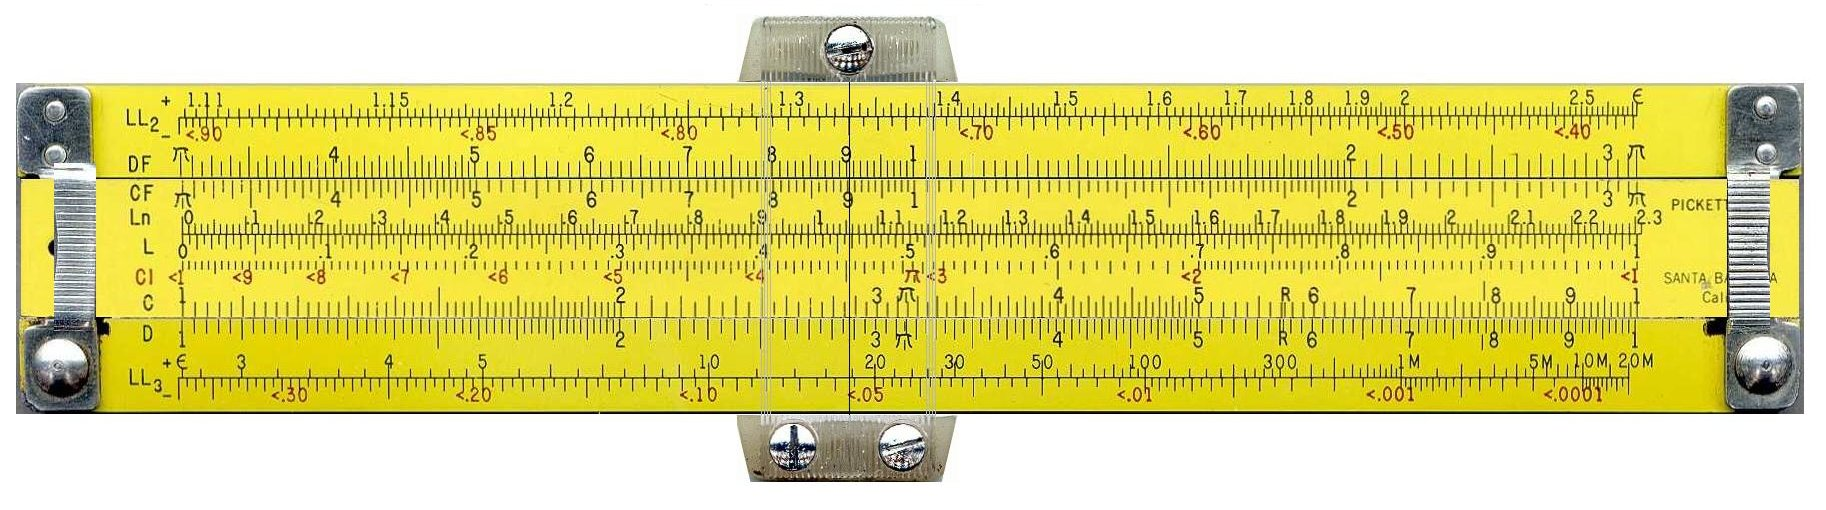
\includegraphics[width=0.93\textwidth]{siber2.jpg}}{{\Sv}iber.}
$$
Le{\nj}iri imaju podeoke sa decimalom i logaritamskom, a {\cv}esto i sa sinusnom skalom.
Jedan od {\nj}ih je bio klizni, te otuda popularno ime {\sl{\sv}iber\/}
(od nema{\cv}kog {\sl Rechen\-schieber\/}). Koristi se jednostavno, pomera{\nj}em
kliza{\cv}a i {\cv}ita{\nj}em vrednosti sa odgovaraju{\cc}e skale.
(Videti za\-da\-tke~\ref{sssec:sibersqrt} i~\ref{sssec:siberpower}.)

Postojale su i kru{\zv}ne varijante, pa i {\dz}epne, gde je
{\dz}epni sat sa logaritmarom i kompasom  bio \navod{iPhone} XIX i prve polovine XX~veka.
$$
\slika{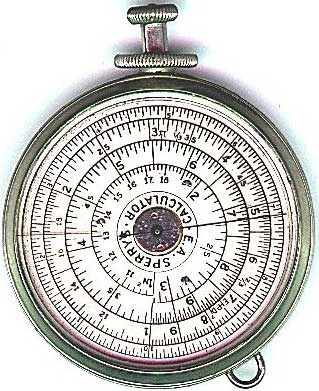
\includegraphics[width=50\mm]{sahat.jpg}}{{\Dz}epni logaritmar.}
$$

Tablice i logaritmari se i danas koriste u vojsci kao rezerva u slu{\cv}aju otkaziva{\nj}a elektronike.
Prvi kompjuter ENIAC (Electronic Numerical Integrator And Computer)
je naprav{\lj}en 1946. godine da bi izra{\cv}unao tablice za vosjku.


%\begin{sideways}%
%$$
%\logaritmar0
%$$
%\end{sideways}

\iffalse
$$
\lambda = 10\cdot\logten\e= {10\over\ln 10}\approx 4\.343.
%=4\.3429448190\,3251827651\,1289189166\,0508229439\,7005803667.
$$


$$
\ln(x)={\lambda\cdot\logten(x)\over 10}.
$$
\fi

\section{Razno}


\subsection{Kompleksni logaritam}

Ako u kompleksnoj ravni imamo kompleksan broj $z\in{\mathbb C}$, 
$$
\slika{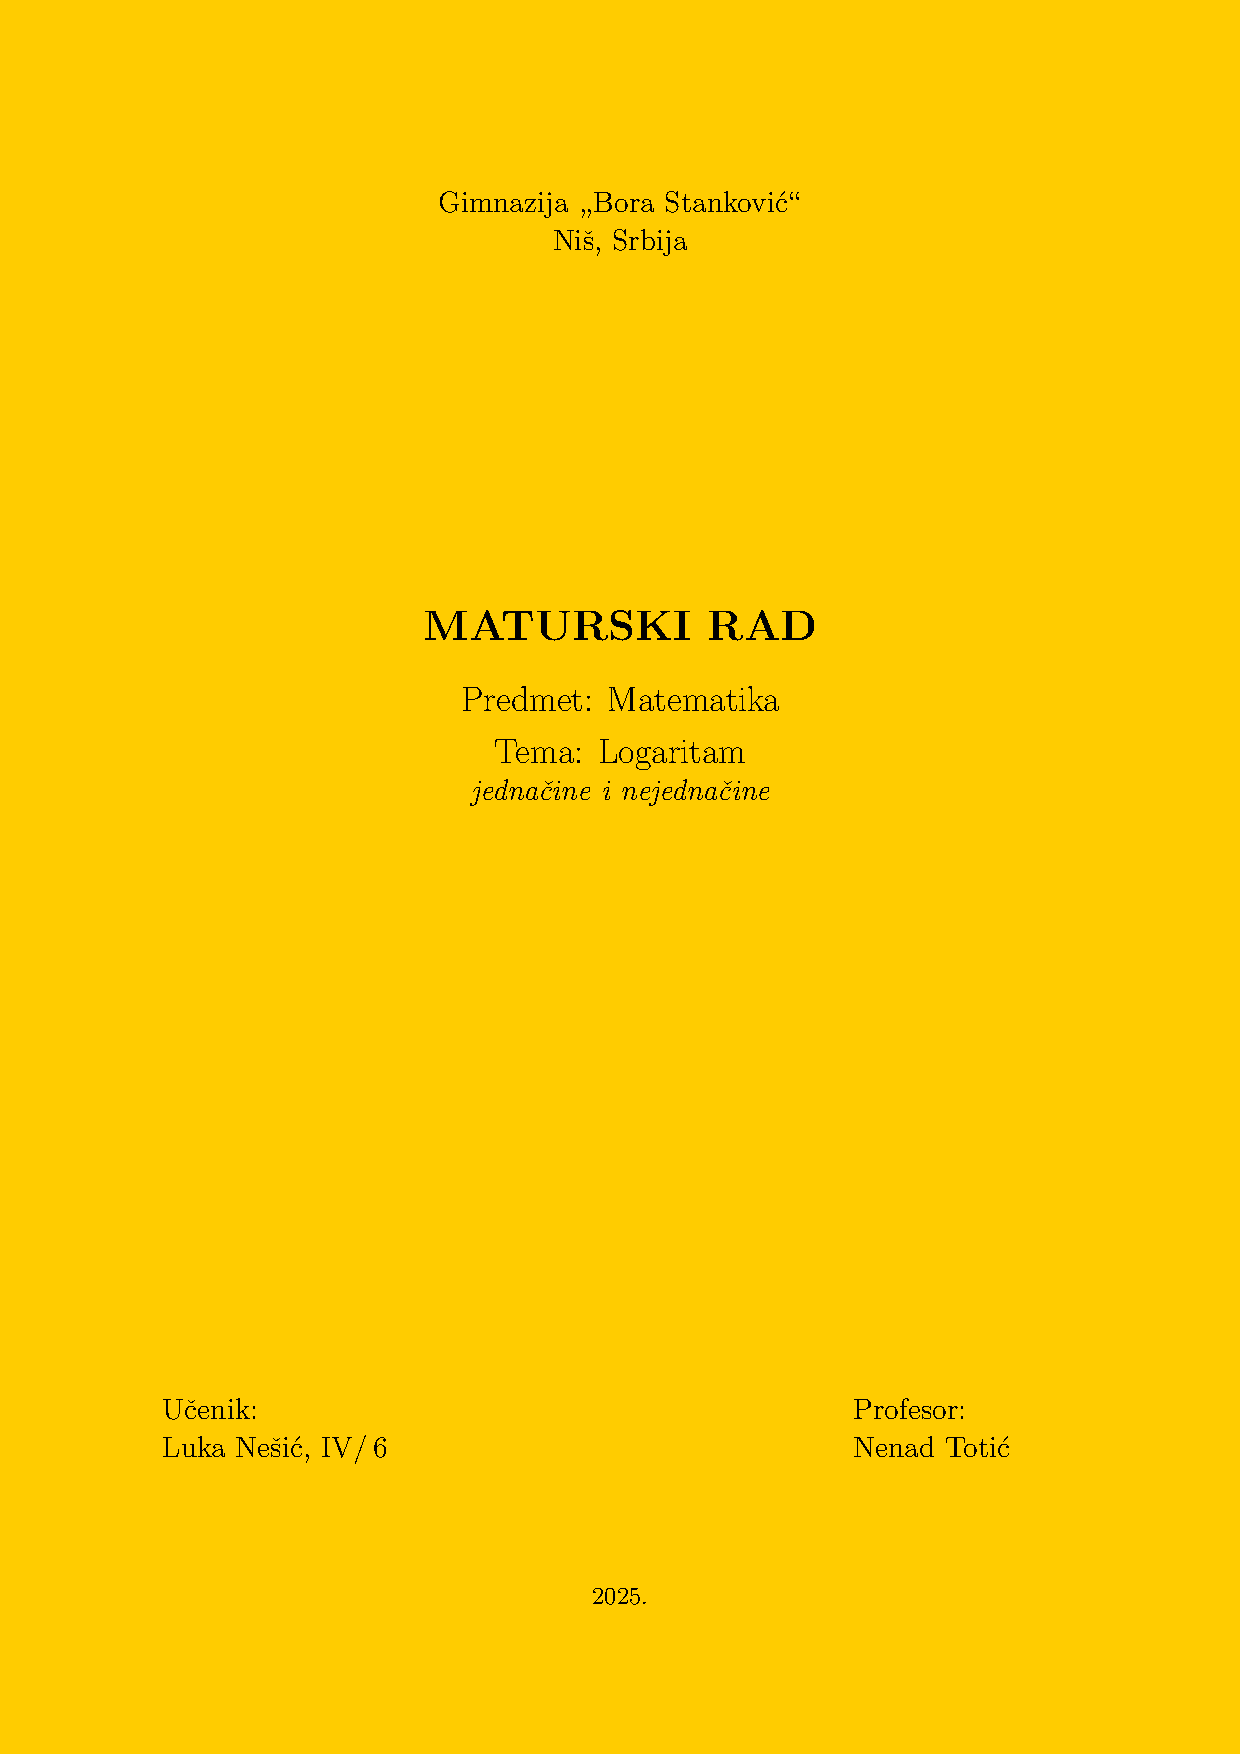
\includegraphics[]{log.2}}{Broj $z$ u kompleksnoj ravni.}
$$
koji mo{\zv}e biti predstav{\lj}ean kao
\begin{alignat*}{3}
z 
&= x + iy &&\qquad\text{pravougle koordinate}\\
&= \rho\, (\cos\theta +i\sin\theta)&&\qquad\text{polarne koordinate}\\
%&= \rho\mathbin{\rm cis}\theta&&\qquad\text{skra{\cc}eni polarni zapis}\\
& = \rho\, \e^{i\theta}&&\qquad\text{Ojlerova formula}
\end{alignat*}
onda se, iz Ojlerove formule i jednakosti \eqref{eq:lnmul} i \eqref{eq:powb}, dobija
\begin{equation}
\okvir{\ln z = \ln\rho + i\theta}.
\label{eq:cln}
\end{equation}
Po{\sv}to je $\rho=|z|=\sqrt{x^2+y^2}\ge0$,
sledi da prirodni logaritam kompleksnog broja $z$ nije definisan ($\rsinfty$) samo za $z=0$.
Kako je $y/x=\tan\theta$, prirodni logaritam kompleksnog broja,
pred\-stav\-{\lj}e\-nog pravouglim koordinatama, iz formule \eqref{eq:cln},
mo{\zv}e se izra{\cv}unati
\begin{equation}
\okvir{\ln(x+iy)={1\over2}\ln(x^2+y^2)+i\arctan\left({y\over x}\right)}.
\label{eq:clncart}
\end{equation}
I za kompleksne brojeve va{\zv}i jednakost promene baze \eqref{eq:chgbase}, tako da za dva kompleksna
broja $z$ i $w$, gde je $z\ne0$, $w\ne0$ i $w\ne1$, sledi
$$
\log_w z={\ln z\over \ln w},
$$
gde se $\ln z$ i $\ln w$ ra{\cv}unaju pomo{\cc}u formule \eqref{eq:cln}, odnosno, \eqref{eq:clncart}.
Na primer,
$$
\log_{2+i}(3+4i)=2, \qquad \log_i\e=-\frac{2i}{\pi}.
$$

\medskip

Iz Ojlerove formule se mo{\zv}e dobiti, kako je nazvana, 
{\sl najlep{\sv}a formula u istoriji ma\-te\-ma\-ti\-ke},
u kojoj je upotreb{\lj}eno 5 najva{\zv}nijih konstatnti u matematici 
($0,1,\pi,\e,i$)
$$
\okvir{\e^{i\pi}+1=0},
$$
gde, ako prebacimo 1 na desnu stranu i {\sl logaritmujemo}, dobijamo zanim{\lj}iva jednakost
$$
{\ln(-1)\over\sqrt{-1}}=\pi.
$$

Jo{\sv} jedna zanim{\lj}iva jednakost se mo{\zv}e dobiti pomo{\cc}u kompleksnog logaritma, a to je
vrednost $i^{\,i}$.
Kako $i$ ima polarne koordinate $\rho=1$ i $\theta=\pi/2$, ako ga predstavimo Ojlerovom formulom kao
$i=\e^{i\pi/2}$ i iz jednakosti \eqref{eq:power} i \eqref{eq:powb}, sledi da je
$$
i^{\,i}=\e^{i\ln i} = \e^{i\ln \e^{i\pi/2}}=\e^{i^2\pi/2}=\e^{-\pi/2}\approx0.20788 
$$
realan broj.

\subsection{Izvod}


Ako je 
$$
y=\ln x\sledi y'={1\over x},
$$
odakle se, pomo{\cc}u jednakosti \eqref{eq:chgbase} i jednakosti za izvod slo{\zv}ene funkcije, mo{\zv}e dobiti
\begin{equation}
\okvir{y=\logb(f(x))\sledi y'={f'(x)\over f(x)\ln b}}.
\label{eq:izvod}
\end{equation}

\def\dx{{\it dx}}
Povr{\sv}ina figure ispod funkcije $y=1/x$ do $x$-ose, u opsegu od 1~do~$x$ iznosi 
$\ln x$.\penalty-1000
(Matemati{\cv}ki zapisano: $\int_1^x\dx/x=\ln x$.)
$$
\slika{\includegraphics[]{izvod.3}}{Geometrijsko zna{\cv}e{\nj}e $\ln x$.}
$$
(Na slici je $x=\e$, tako da je povr{\sv}ina osen{\cv}ane figure jednaka 1.)

\subsection{Limes}

Ojler je dokazao da je
$$
\ln x=\lim_{n\to\infty}n(\sqrt[n]x-1).
$$

\subsection{Teorema prostih brojeva}

Jo{\sv} jedno mesto gde se pojav{\lj}uje prirodni logaritam u {\sl teoriji brojeva} je,
takozvana, {\sl teorema prostih brojeva\/} (PNT), kojom se je bavio Gaus kada je
imao samo 15--16 godina.

\smallskip

Ako funkcija $\pi(n)$ ima vrednost {\sl ukupan broj prostih brojeva ma{\nj}ih
ili jednakih od~$n$}, onda va{\zv}i
$$
\lim_{n\to\infty}{\pi(n)\ln n\over n} = 1.
$$
Posledica ove teoreme je da je $n$-ti prost broj, za veliko $n$, otprilike
$$
p_n\approx n\ln n.
$$


\section{Zadaci}

\def\jed#1{Jedna{\cv}ina~#1}


\subsection{\jed1}

\zad Na{\dj}i re{\sv}e{\nj}e jedna{\cv}ne
$$
\log_2(x-2)+\log_4(x-2)+\log_{16}(x-2)=7.
$$
(Zadatak sa mog prijemnog ispita na FIT.)

\ans
Vidimo da su osnove logaritama stepeni broja 2, 
pa iz jednakosti za logaritam stepena osnove \eqref{eq:powbase} sledi
\begin{align*}
\log_2(x-2)+\log_{2^2}(x-2)+\log_{2^4}(x-2)&=\\
\log_2(x-2)+{1\over2}\log_2(x-2)+{1\over 4}\log_2(x-2)&=\\
\noalign{\smallskip}
{7\over4}\log_2(x-2)&=7,
\intertext{odnosno, posle skra{\cc}iva{\nj}a,}
\log_2(x-2)&=4.
\end{align*}
Odavde je
$$
x-2=2^4=16\sledi
x=\ram{18}.
$$

\subsection{\jed2}

\zad
Re{\sv}i jedna{\cv}inu
$$
2\log(x) - \log(6-x)=0.
$$

\ans
Da bi logaritam u jedna{\cv}ini bio definisan mora biti 
$$
x>0\land 6-x>0\sledi 0<x<6.
$$
Zbog jednakosti \eqref{eq:bpow} mo{\zv}emo pisati
\begin{align*}
\log(x^2)&=\log(6-x)
\intertext{odakle sledi}
x^2&=6-x\\
x^2+x-6&=0.
\end{align*}
Re{\sv}ava{\nj}em kvadratne jedna{\cv}ine
\begin{align*}
x_{1,2}&={-1\pm\sqrt{1^2+4\cdot1\cdot6}\over2\cdot1}\\
&={-1\pm\sqrt{25}\over2}\\
&={-1\pm5\over2},
\intertext{dobijamu re{\sv}e{\nj}a $x_1=2$ i $x_2=-3$, odakle je jedinstveno re{\sv}e{\nj}e}
x&=\ram{2}.
\end{align*}

\subsection{\jed3}

\zad
Re{\sv}i jedna{\cv}inu
$$
\ln(x)=\ln(15-x)-\ln(x+1).
$$

\ans
Jedna{\cv}ina je definisana za
$$
x>0\land 15-x>0\land x+1>0\sledi 0<x<15.
$$
Ako zapi{\sv}emo jedna{\cv}inu kao
\begin{align*}
\ln(x)+\ln(x+1)&=\ln(15-x)
\intertext{iz jednakosti za logaritam proizvoda \eqref{eq:lnmul}, mo{\zv}emo pisati}
\ln(x (x+1)) &= \ln(15-x)\\
\ln(x^2+x)&=\ln(15-x)\\
x^2+x&=15-x\\
x^2+2x-15&=0
\end{align*}
Re{\sv}ava{\nj}em kvadratne jedna{\cv}ine dobijamo 2 re{\sv}e{\nj}a, $x_1=3$ i $x_2=-5$, ali zbog
uslova, ostaje jedinstveno
$$
x=\ram{3}.
$$


\subsection{Geometrijski niz}

\zad
Za $0\le x<1$, uprostiti izraz
$$
y=\log(1+x+x^2+x^3+x^4+\cdots).
$$

\ans
Kako je zbir\footnote{{\bf Dokaz:} Ako je $s=1+x+x^2+x^3+x^4+\cdots=1+x\cdot(1+x+x^2+x^3+x^4+\cdots)
=1+x\cdot s$, onda sledi $s=1/(1-x)$. \QED} beskona{\cv}nog geometrijskog niza
$$
1+x+x^2+x^3+x^4+\cdots = {1\over 1-x},
$$
mo{\zv}e se pisati
\begin{align*}
\noalign{\vskip-12pt}
y&=\log\left({1\over 1-x}\right),
\intertext{gde iz jednakosti za recipro{\cv}nu vrednost \eqref{eq:recip}, sledi}
&=\ram{-\log(1-x)}.
\end{align*}

\subsection{Poluraspad joda}

\def\iso#1-#2{\vphantom{\rm#2}^{#1}{\rm#2}}

\zad 
Ako imamo $63\um g$ izotopa joda $\iso 131-I$, a znamo da smo pre 11 dana imali $163\um g$, koje je vreme
poluraspada ovog izotopa? (Koristi prirodni logaritam.)

\ans
Iz formule \eqref{eq:halftime} na strani \pageref{eq:halftime}, sledi da se vreme poluraspada
mo{\zv}e izra{\cv}unati
$$
\th
={t\over \logtwo(m_0 / m_t)}
={t\ln2\over \ln(m_0 / m_t)}
%={11\over\logtwo(163/63)}
={11\ln2\over\ln(163/63)}
\approx\ram{8.02\um{dana}}.
$$



%\clearpage

\subsection{Beskona{\cv}ni koren}

\zad
Odredi vrednost
$$
x=\ln\left(\e\sqrt[2]{\e\sqrt[3]{\e\sqrt[4]{\e\sqrt[5]{\cdots}}}}\right)
$$
gde je $\e$ osnova prirodnog logaritma.

\ans Kako je $\ln \e=1$, a koriste{\cc}i jednakost za logaritam proizvoda \eqref{eq:lnmul} 
i jednakost za logaritam korena \eqref{eq:lnroot},  mo{\zv}emo pisati
\begin{align*}
x
&=\ln\left(\e\sqrt[2]{\e\sqrt[3]{\e\sqrt[4]{\e\sqrt[5]{\cdots}}}}\right)\\
&=1+\frac12\ln\left(\e\sqrt[3]{\e\sqrt[4]{\e\sqrt[5]{\cdots}}} \right)\\
&=1+\frac12\left(1+\frac13\ln\left(\e\sqrt[4]{\e\sqrt[5]{\cdots}} \right)\right)\\
&=1+\frac12\left(1+\frac13\left(1+\frac14\ln\left(\e\sqrt[5]{\cdots} \right) \right)\right)\\
&=1+\frac12\left(1+\frac13\left(1+\frac14\left(1+\frac15\ln(\cdots)\right) \right) \right)\\
&=1+\frac12+\frac12\mul\frac13+\frac12\mul\frac13\mul\frac14+\frac12\mul\frac13\mul\frac14\mul\frac15+\cdots\\
&={1\over\ep1!}+{1\over\ep2!}+{1\over\ep3!}+{1\over\ep4!}+{1\over\ep5!}+\cdots
\intertext{Ako pogledamo formulu \eqref{eq:e} na strani \pageref{eq:e}, mo{\zv}emo videti da je ovaj zbir jednak}
x&=\ram{\e-1},
\end{align*}
jer iz sume za izra{\cv}unava{\nj}e $\e$ nedostaje {\sl nulti\/} {\cv}lan $1/0!=1$.


\subsection{Decimalne cifre}
\zad Koliko decimalnih cifara ima 128-bitna promen{\lj}iva?
\ans $d=\lfloor\logten 2^{128}\rfloor+1=\lfloor 128\logten 2\rfloor+1=\lfloor 38.5318\rfloor+1=38+1=\ram{39}.$


\subsection{Izvod}
\zad Odredi izvod funkcije $f(\alpha)=\log_3(\cos\alpha)$.
\ans Kako je izvod $\cos\alpha$ jednak $-\sin\alpha$ i iz jednakosti 
za izvod logaritma funkcije \eqref{eq:izvod}, sledi da je
$$
f'(\alpha)
={-\sin\alpha\over\cos\alpha\ln3}
%\noalign{\smallskip}
=\ram{-{\tan\alpha\over\ln3}}.
$$

\clearpage

\subsection{{\Cv}etiri {\cv}etvorke}

\def\4{{\color{red}\bf4}}

\zad
Dokazati da svaki prirodan broj $n\in{\mathbb N}$, mo{\zv}e biti predstav{\lj}en sa \4 broja \4,
pomo{\cc}u logaritamske funkcije i kvadratnog korena
$$
n=\log_{\sqrt\4/\4}\left(\log_\4 \underbrace{\sqrt{\sqrt{\cdots\sqrt\4}}}_{\text{$n$ korena}}\right).
$$

\ans
Kako je
$$
{\sqrt \4\over \4}={1\over2}
\qquad\text{i}\qquad
\underbrace{\sqrt{\sqrt{\cdots\sqrt \4}}}_{\text{$n$ korena}}=\4^{(1/2)^n},
$$
izraz mo{\zv}e biti upro{\sv}{\cc}en
\begin{align*}
\noalign{\vskip-9pt}
\log_{\sqrt\4/\4}\left(\log_\4 \underbrace{\sqrt{\sqrt{\cdots\sqrt\4}}}_{\text{$n$ korena}} \right)
&=\log_{1/2}\left(\log_\4 \4^{(1/2)^n}\right),\\
\intertext{gde iz jednakosti za logaritam stepena osnove \eqref{eq:powb}, sledi}
&=\log_{1/2}(1/2)^n\\
&=\ram{n}.
\end{align*}

\def\2{{\it2}}
\def\dlog{\mathop{\sl\ell og}\nolimits_\2}
\begingroup\it
Davno je u jednom {\cv}asopisu postav{\lj}en sli{\cv}an zadatak: 
da se sa {\sv}to ma{\nj}e istih brojeva,
koriste{\cc}i bilo koju matemati{\cv}ku funkciju, predstavi 
svaki prirodan broj $n$.
Re{\sv}io ga je nobelovac Pol Dirak (Paul Dirac) 
sa~3~broja~\2, {\cv}ije originalno
re{\sv}e{\nj}e izgleda
$$
%n=
-\dlog\dlog\sqrt{\cdots n\cdots\sqrt\2}
=-\dlog\dlog\2^{\2^{-n}}
=-\dlog\2^{-n}=n.
\eqno{\square}$$
\endgroup


\subsection{ln 3}\label{sssec:ln3}
 
\zad
Pomo{\cc}u postupka \eqref{eq:alg} sa 
strane~\pageref{eq:alg},
izra{\cv}unati {\sl pe{\sv}ke\/} pribli{\zv}nu vrednost $\ln 3$, 
u~5 koraka. Za upore{\dj}iva{\nj}e, ta{\cv}na vrednost je
$$
\ln3=1\.
0986122886\,
6810969139\,
5245236922\,
5257046475\,\ldots
%1639157/1492025=1.098612288668
$$

\def\step#1{\par\smallskip\indent\leavevmode
  Korak {\it#1}.\kern2em\relax}

\ans
Za $x=3$, izraz $r=(x-1)/(x+1)=1/2$. U nultom koraku postav{\lj}amo po{\cv}etne vrednosti:
\step0 $k=1,\quad p=2r=1,\quad q=r^2=1/4,\quad a=p=1,\quad y=a=1$.

\smallskip
\noindent Slede koraci iteracije --- pove{\cc}amo $k$ za 2, pomno{\zv}imo $p$ sa $q$,
{\cv}lan sume $a$ postaje $p/k$, koga dodajemo u rezultat $y$:

\step1 $k=3,\quad p=1/4,\quad a=1/12,\quad y=13/12$;
\step2 $k=5,\quad p=1/16,\quad a=1/80,\quad y=263/240$;
\step3 $k=7,\quad p=1/64,\quad a=1/448,\quad y=7379/6720$;
\step4 $k=9,\quad p=1/256,\quad a=1/2304,\quad y=88583/80640$;
\step5 $k=11,\quad p=1/1024,\quad a=1/11264,\quad y=3897967/3548160$.

\medskip
\noindent Rezultat je
$$
\ln3\approx{3897967\over3548160}\approx \ram{1\.0986},
$$

\smallskip\noindent
{\sv}to je prili{\cv}no ta{\cv}no za samo 5 koraka, jer je apsolutna gre{\sv}ka oko $2\.4\puta10^{-5}$.
%Kada bi smo ra{\cv}unali u 20 koraka, 
%dobili bi smo $y={636083906982236368109838473\over578988523561291667944243200}$, 
%gre{\sv}ka bi bila oko $7\puta10^{-15}$, {\sv}to je preciznost s kojom je 1617.\ godine Brigs (Henry Briggs)
%izra{\cv}unao svoje {\sl logaritamske tablice}.


\subsection{Analogni kvadratni koren}\label{sssec:sibersqrt}

\zad
Objasni na{\cv}in za odre{\dj}iva{\nj}e vrednosti $\sqrt x$ logaritmarom.

\ans Kvadratni koren se mo{\zv}e direktno {\cv}itati sa logaritmara ako {\sl u glavi\/} izvr{\sv}imo 
de{\lj}enje sa 2, i po potrebi, sabira{\nj}e sa $0\.5$, 
{\sv}to je vrlo jednostavno, jer se radi o brojevima izme{\dj}u 0 i 1 sa najvi{\sv}e 3 decimale. 
Kako je
$$
\sqrt x=10^{{1\over2}\log x},
$$
potrebno je odrediti vrednost $\log x$, a onda za dvostruko ma{\nj}u vred\-nost od {\nj}e, pro{\cv}itati vrednost $10^y$. Na primer,
za izra{\cv}unava{\nj}e $\sqrt{5\.3}$,
{\cv}itamo da je $\log 5\.3\approx0\.724$, a onda {\cv}itamo vrednost $10^y$ za 
$y=0\.724/2=0\.362$ i
dobijamo $\sqrt{5\.3}\approx 2\.3$.
$$
\def\hair{\nit{0.36213793480039452281649614581363}\nit{0.72427586960078904563299229162726}\nit{0.86213793480039452281649614581363}}
\def\extra{\ruler{0.36213793480039452281649614581363}{$\uparrow$}\ruler{0.72427586960078904563299229162726}{$\downarrow$}\ruler{0.86213793480039452281649614581363}{$\uparrow$}}
\logaritmar0
$$
Za $\sqrt{53}$ treba u $y$ dodati jo{\sv} $0\.5$ tako da je $y=0\.362+0\.5=0\.862$, odakle je $\sqrt{53}\approx7\.28$.
%(Dodava{\nj}e $0\.5$ u eksponent predstav{\lj}a mno{\zv}e{\nj}e celog izraza sa $\sqrt{10}$.)
Naravno, $\sqrt{530}$ se ra{\cv}una kao $10\sqrt{5\.3}$, ili $\sqrt{0\.53}={1\over10}\sqrt{53}$.

\subsection{Analogni stepen}\label{sssec:siberpower}

\zad
Odredi logaritmarom pribli{\zv}nu vrednost
$z=2\.3^{1\.7}$.

\ans
Pomo{\cc}u jednakosti \eqref{eq:power} predstavimo
$$
z=2\.3^{1\.7}=10^{1\.7\cdot\log(2\.3)}.
$$
Prvo odre{\dj}ujemo vrednost $\log(2\.3)$ tako {\sv}to nalazimo
$x=2\.3$ i {\cv}itamo ispod {\nj}ega vred\-nost $\log x$ (vidi nit obele{\zv}enu sa `{\color{red}
$\updownarrow$}').
$$
\def\hair{\nit{0.36172783601759287886777711225119}}
\def\extra{\ruler{0.36172783601759287886777711225119}{$\updownarrow$}}
\logaritmar0
$$
Nalazimo da je $\log(2\.3)\approx0\.362$. Nakon toga, tu vrednost na kliza{\cv}u poravnavamo sa $x=1$.
Kako na kliza{\cv}u ne postoji $0\.362$, postavi{\cc}emo na $3\.62$, s tim {\sv}to {\cc}emo rezultat
podeliti sa 10. Sada, za $x=1\.7$ {\cv}itamo vrednost na kliza{\cv}u ispod
$$
\def\hair{\nit{0.55838193028134245441924844418993}\nit{0.78883085165961638295941833851827}\nit{1.173319251511250348494469535017}}
\def\extra{\ruler{0.55838193028134245441924844418993}{$\uparrow$}\ruler{1.173319251511250348494469535017}{$z$}%
\ruler{0.78883085165961638295941833851827}{$\uparrow$}}
\logaritmar{-0.55838193028134245441924844418993}
$$
i nalazimo da je oko $6\.15$, {\sv}to zna{\cv}i da je $1\.7\cdot\log(2\.3)\approx0\.615$.
\iffalse
Vra{\cc}amo kliza{\cv} u po{\cv}etni polo{\zv}aj i {\cv}itamo koja je vrednost na 
kliza{\cv}u iznad $\log x=0\.615$, odnosno, koliko je $10^{0\.615}$.
$$
\def\hair{\nit{0.61493732122990789407522109082702}}
\def\extra{\ruler{0.61493732122990789407522109082702}{$\updownarrow$}}
\logaritmar0
$$
\else
Nakon toga, za $y=0\.615$ {\cv}itamo vrednost $10^y$.
\fi
Nalazimo da je oko $4\.12$ {\sv}to je i re{\sv}e{\nj}e
$$
z=2\.3^{1\.7} \approx \ram{4\.12},
$$
a ta{\cv}na vrednost je $z=4\.120380\ldots$


\section{Reference}

\subsection{Literatura}

%\nocite{*}%
%\renewcommand{\refname}{}%

%\printbibliography

\def\lit#1#2#3(#4){\item 
#1: \navod{#2}, {\sl#3\/} (#4)}
\renewcommand{\labelenumi}{[{\it\arabic{enumi}\/}]}

\begin{enumerate}
\lit{Larousse}{Matematika}{Op{\sv}ta enciklopedija}(1967)
\lit{Neboj{\sv}a Ikodinovi{\cc}, Sla{\dj}ana Dimitrijevi{\cc}, Suzana Aleksi{\cc}}{U{\dz}benik sa
zbirkom zadataka za 2. razred gimnazije}{Matematika 2}(2019)
\lit{Vene Bogoslavov}{Zbirka re\sv enih zadataka iz matematike 2}{}(2008--2011)
\lit{Marjan Mateji\cc, Lidija Stefanovi\cc, Branislav Ran\dj elovi\cc, Igor Milovanovi\cc}{Kom\-ple\-ti
zadataka za prijemni ispit}{Matematika}(2011)
\lit{Rade Nikoli{\cc}}{Zadaci za prijemni ispit iz matematike na Fakultet informacionih tehnologija}{}(2020)
\lit{Gradimir V. Milovanovi{\cc}, {\Dj}or{\dj}e R. {\Dj}or{\dj}evi{\cc}}{Programira{\nj}e numeri{\cv}kih metoda}{}(1981)
\lit{Donald E. Knuth}{Seminumerical Algorithms}{The Art of Computer Programming}(1968--)
\lit{Drago{\lj}ub Vasi{\cc}, Vene Bogoslavov, Gli{\sv}a Ne{\sv}kovi{\cc}}{Logaritamske tablice}{}(2008)
\lit{Henry Briggs}{Arithmetica logarithmica}{}(1624)
\end{enumerate}

\subsection{Linkovi}

\def\link#1#2{\item\href{#1}{#2\hfill\break{\footnotesize\tt#1}}}

\begin{enumerate}
\link{https://en.wikipedia.org/wiki/Logarithm}{{\sc WikipediA} --- Logarithm}
\link{https://mathworld.wolfram.com/Logarithm.html}{Wolfram MathWorld --- Logarithm}
\link{https://mathworld.wolfram.com/Antilogarithm.html}{Wolfram MathWorld --- Antiogarithm}
\link{https://reference.wolfram.com/language/ref/Log.html}{Wolfram Language \& System Documentation Center --- Logarithm}
\link{https://inria.hal.science/inria-00543939/PDF/briggs1624doc.pdf}{A reconstruction of the tables of Briggs' {\sl Arithmetica logarithmica\/} (1624)}
\link{https://people.mpim-bonn.mpg.de/zagier/files/doi/10.2307/2975232/fulltext.pdf}{Newman's Short Proof of the Prime Number Theorem}
\link{https://www.youtube.com/watch?v=VRzH4xB0GdM}{{\sf YouTube} --- Log Tables --- Numberphile}
\link{https://www.youtube.com/watch?v=xRpR1rmPbJE}{{\sf YouTube} --- The iPhone of Slide Rules --- Numberphile}
\link{https://www.youtube.com/watch?v=Noo4lN-vSvw}{{\sf YouTube} --- The Four 4s --- Numberphile}
%\link{https://github.com/Nasumica/Wirth}{GitHub --- Srbislav D. Ne{\sv}i{\cc} --- Numerical recipes in Pascal}
\end{enumerate}


\clearpage

\thispagestyle{empty}


\leavevmode\hbox{}

\vfill

\begin{center}
%\qrcode{https://docs.google.com/viewer?url=$https://github.com/Nasumica/LukaMaturski/blob/main/log.pdf}
\qrcode{https://github.com/Nasumica/LukaMaturski/blob/main/log.pdf}
\end{center}

\end{document}
